\documentclass[xcolor=table]{beamer}

\usepackage{beamerthemeBerkeley}

\usepackage{amsmath}
\usepackage{fontenc}
\usepackage[french]{babel}

\usepackage[utf8]{inputenc}
\usepackage[T1]{fontenc}

\usepackage{graphicx}
\usepackage{calligra}
\usepackage{ulem}
\usepackage{colortbl}

\usepackage[table]{xcolor}
\usepackage{ragged2e}
\setbeamertemplate{blocks}[rounded][shadow=true]

\definecolor{ensimagreen}{RGB}{20,49,67}
\usecolortheme[named=ensimagreen]{structure}
\setbeamercolor{subsection in head/foot}{fg=white, bg=ensimagreen}
\setbeamercolor{section in head/foot}{fg=white, bg=ensimagreen}
\setbeamercolor{normal text}{fg=ensimagreen,bg=white}

\setbeamercolor{logo}{bg=white}
\setbeamertemplate{sidebar canvas right}[vertical shading][top=ensimagreen,middle=ensimagreen,bottom=ensimagreen]
\setbeamercolor{subsection in sidebar}{bg=white,fg=white}
\setbeamercolor{section in sidebar}{bg=ensimagreen,fg=white}
\setbeamertemplate{itemize item}[ball]

%\logo{\includegraphics[scale=0.05]{X2.png}}

\title{}

\date{}
\begin{document}


%\setbeamertemplate{background canvas}{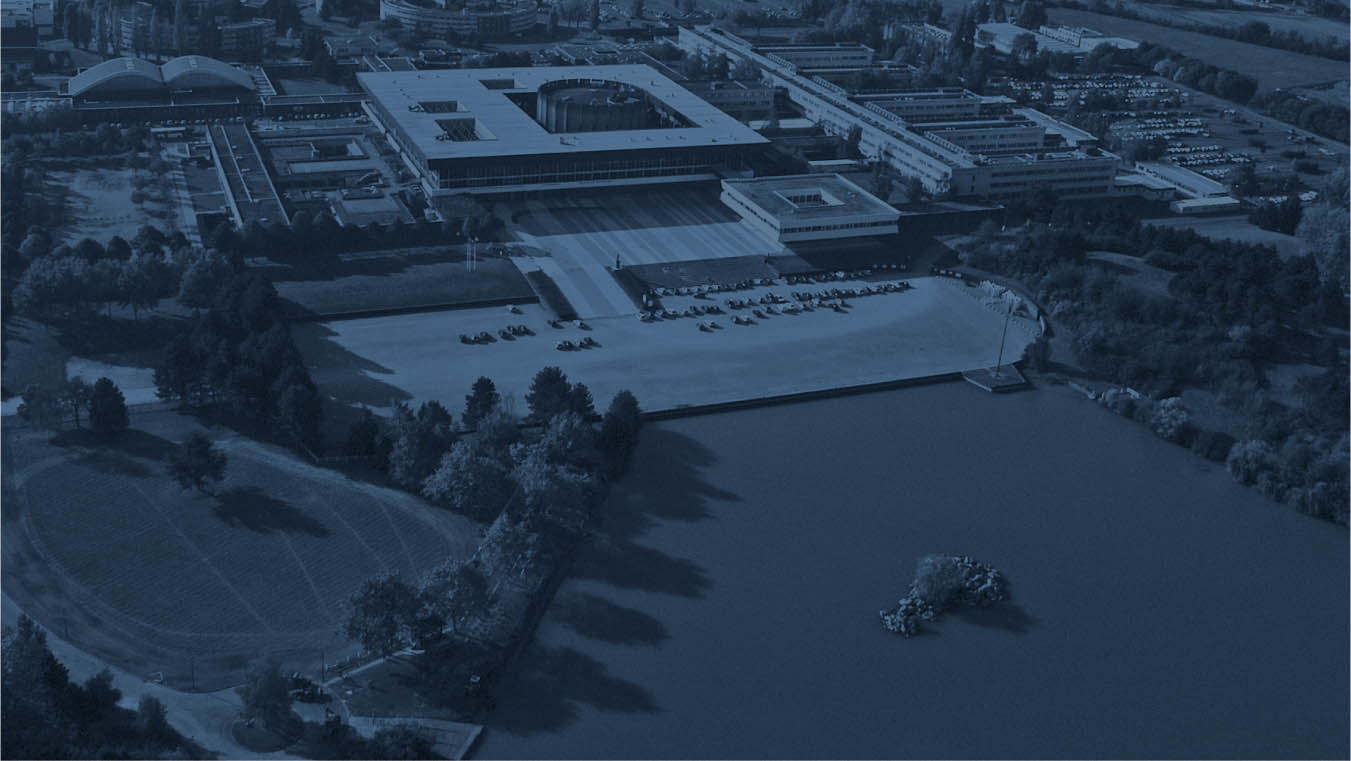
\includegraphics[width=\paperwidth,height=\paperheight]{ecole.png}}
\begin{frame}[plain]


\begin{center}
\textcolor{white}{\Large{Histoire des sciences contemporaines} \\ \bigskip \large{ Au delà de Galois et Poincaré :  \\
créations individuelles et dynamiques collectives}}

\bigskip


\bigskip
\textcolor{white}{\large {Frédéric Brechenmacher}} 

\bigskip
\textcolor{white}{\small{Laboratoire interdisciplinaire de l'X \\ \bigskip Département humanités et sciences sociales \\ École polytechnique}}

\end{center}

\end{frame}

\setbeamertemplate{background canvas}{}


\section{Préambule : un dilemme}
\begin{frame}
\frametitle{Préambule : un dilemme}

\pause
…
\end{frame}



\end{document}